\documentclass[a4paper,10pt]{article}
\usepackage[utf8]{inputenc}
%\usepackage{nips01e}
\usepackage{amsfonts}
%\usepackage{harvard}
\usepackage{amsmath}
\usepackage{fullpage}
%\usepackage[dutch]{babel}
%\usepackage[subnum]{cases}
\usepackage{amssymb}
%\usepackage{psfrag}
\usepackage{graphicx}
\usepackage{fancyhdr,color}
%\usepackage{mcode}
\usepackage{hyperref}





% section added by EE227AT
%
% Definitions and macros
%

%\setlength{\marginparwidth}{1.2in}
%\let\oldmarginpar\marginpar
%\renewcommand\marginpar[1]{\-\oldmarginpar[\raggedleft\footnotesize #1]%
%{\raggedright\footnotesize #1}}

%\renewcommand{\indexspace}{\rule{0cm}{.4cm}}
%% end example/remark
%\newcommand{\eex}{\ifmmode\sq\else{\unskip\nobreak\hfil
%  \penalty50\hskip1em\null\nobreak\hfil$\Diamond$
%  \parfillskip=0pt\finalhyphendemerits=0\endgraf}\fi{}}
%\newcommand{\erem}{\ifmmode\sq\else{\unskip\nobreak\hfil
%  \penalty50\hskip1em\null\nobreak\hfil$\star$
%  \parfillskip=0pt\finalhyphendemerits=0\endgraf}\fi{}}
%\newcommand{\eobs}{\ifmmode\sq\else{\unskip\nobreak\hfil
%  \penalty50\hskip1em\null\nobreak\hfil$\vartriangleleft$
%  \parfillskip=0pt\finalhyphendemerits=0\endgraf}\fi{}}

% VET - characters - lowercase
\newcommand{\avet}{{\mathbf  a}}
\newcommand{\bvet}{{\mathbf  b}}
\newcommand{\cvet}{{\mathbf  c}}
\newcommand{\dvet}{{\mathbf  d}}
\newcommand{\evet}{{\mathbf  e}}
\newcommand{\fvet}{{\mathbf  f}}
\newcommand{\gvet}{{\mathbf  g}}
\newcommand{\hvet}{{\mathbf  h}}
\newcommand{\ivet}{{\mathbf  i}}
\newcommand{\jvet}{{\mathbf  j}}
\newcommand{\kvet}{{\mathbf  k}}
\newcommand{\lvet}{{\mathbf  l}}
\newcommand{\mvet}{{\mathbf  m}}
\newcommand{\nvet}{{\mathbf  n}}
\newcommand{\ovet}{{\mathbf  o}}
\newcommand{\pvet}{{\mathbf  p}}
\newcommand{\qvet}{{\mathbf  q}}
\newcommand{\rvet}{{\mathbf  r}}
\newcommand{\svet}{{\mathbf  s}}
\newcommand{\tvet}{{\mathbf  t}}
\newcommand{\uvet}{{\mathbf  u}}
\newcommand{\vvet}{{\mathbf  v}}
\newcommand{\xvet}{{\mathbf  x}}
\newcommand{\yvet}{{\mathbf  y}}
\newcommand{\zvet}{{\mathbf  z}}
\newcommand{\wvet}{{\mathbf  w}}

% VET - characters - uppercase
\newcommand{\Avet}{{\mathbf  A}}
\newcommand{\Bvet}{{\mathbf  B}}
\newcommand{\Cvet}{{\mathbf  C}}
\newcommand{\Dvet}{{\mathbf  D}}
\newcommand{\Evet}{{\mathbf  E}}
\newcommand{\Fvet}{{\mathbf  F}}
\newcommand{\Gvet}{{\mathbf  G}}
\newcommand{\Hvet}{{\mathbf  H}}
\newcommand{\Ivet}{{\mathbf  I}}
\newcommand{\Jvet}{{\mathbf  J}}
\newcommand{\Kvet}{{\mathbf  K}}
\newcommand{\Lvet}{{\mathbf  L}}
\newcommand{\Mvet}{{\mathbf  M}}
\newcommand{\Nvet}{{\mathbf  N}}
\newcommand{\Ovet}{{\mathbf  O}}
\newcommand{\Pvet}{{\mathbf  P}}
\newcommand{\Qvet}{{\mathbf  Q}}
\newcommand{\Rvet}{{\mathbf  R}}
\newcommand{\Svet}{{\mathbf  S}}
\newcommand{\Tvet}{{\mathbf  T}}
\newcommand{\Uvet}{{\mathbf  U}}
\newcommand{\Xvet}{{\mathbf  X}}
\newcommand{\Yvet}{{\mathbf  Y}}
\newcommand{\Vvet}{{\mathbf  V}}
\newcommand{\Wvet}{{\mathbf  W}}
\newcommand{\Zvet}{{\mathbf  Z}}

\newcommand{\Deltavet}{\mathbf  \Delta}
\newcommand{\Lambdavet}{{\mathbf  \Lambda}}
\newcommand{\Sigmavet}{\mathbf  \Sigma}
\newcommand{\Thetavet}{{\mathbf  \Theta}}

% Special characters:
\newcommand{\s}{ {\sigma} }

\newcommand{\e}{{\mathrm e}}
\newcommand{\jm}{{\mathrm j}}
\newcommand{\E}{{\mathrm E}}
\newcommand{\Ex}{{\mathbb E}}
\renewcommand{\d}{{\mathrm d}}
\newcommand{\dt}{{\mathrm d}t}
\newcommand{\X}{ {\mathcal X} }
\newcommand{\Y}{ {\mathcal Y} }
\newcommand{\Z}{ {\mathcal Z} }



\newcommand{\calA}{{\mathcal A}}
\newcommand{\calB}{{\mathcal B}}
\newcommand{\calC}{{\mathcal C}}
\newcommand{\calD}{{\mathcal D}}
\newcommand{\calE}{{\mathcal E}}
\newcommand{\calF}{{\mathcal F}}
\newcommand{\calG}{{\mathcal G}}
\newcommand{\calH}{{\mathcal H}}
\newcommand{\calI}{{\mathcal I}}
\newcommand{\calJ}{{\mathcal J}}
\newcommand{\calK}{{\mathcal K}}
\newcommand{\calL}{{\mathcal L}}
\newcommand{\calM}{{\mathcal M}}
\newcommand{\calN}{{\mathcal N}}
\newcommand{\calO}{{\mathcal O}}
\newcommand{\calP}{{\mathcal P}}
\newcommand{\calQ}{{\mathcal Q}}
\newcommand{\calR}{{\mathcal R}}
\newcommand{\calS}{{\mathcal S}}
\newcommand{\calT}{{\mathcal T}}
\newcommand{\calU}{{\mathcal U}}
\newcommand{\calV}{{\mathcal V}}
\newcommand{\calX}{{\mathcal X}}
\newcommand{\calY}{{\mathcal Y}}
\newcommand{\calW}{{\mathcal W}}
\newcommand{\calZ}{{\mathcal Z}}
\newcommand{\qtil}{{\tilde{q}}}
\newcommand{\td}{{\tilde{\delta}}}

\newcommand{\vect}[1]{ {\mbox{\rm vec}(#1)} }

% Macro comandi:

\newcommand{\Atil}{\tilde{A}}
\newcommand{\Zhat}{\hat{Z}}
\newcommand{\Hbar}{\bar{H}}
\newcommand{\Dhat}{\hat{D}}
\newcommand{\dhat}{\hat{d}}
%

\newcommand{\rhat}{\hat{r}}
\newcommand{\xhat}{\hat{x}}
\newcommand{\yhat}{\hat{y}}
\newcommand{\zhat}{\hat{z}}
\newcommand{\xbar}{\bar{x}}
\newcommand{\ubar}{\bar{u}}
\newcommand{\ybar}{\bar{y}}
\newcommand{\zbar}{\bar{z}}
%
\newcommand{\pdot}{\dot{p}}
\newcommand{\pddot}{\ddot{p}}
\newcommand{\pbar}{\bar{p}}
%
\newcommand{\qdot}{\dot{q}}
\newcommand{\qddot}{\ddot{q}}
\newcommand{\qbar}{\bar{q}}
%
\newcommand{\xdot}{\dot{x}}
\newcommand{\ydot}{\dot{y}}
\newcommand{\zdot}{\dot{z}}
\newcommand{\yddot}{\ddot{y}}
\newcommand{\thdot}{\dot{\theta}}
\newcommand{\thddot}{\ddot{\theta}}
\newcommand{\util}{{\tilde{u}}}
\newcommand{\xtil}{{\tilde{x}}}
\newcommand{\ytil}{{\tilde{y}}}
\newcommand{\lam}{\lambda}
\newcommand{\lamax}{\lambda\ped{max}}
\newcommand{\lamin}{\lambda\ped{min}}
%
\newcommand{\adj}{ {\mbox{\rm adj}\;} }
\newcommand{\sign}{\mbox {\rm sgn}}
\newcommand{\spn}{\mbox {\rm span}}
\newcommand{\barJ}{\bar{J}}
\newcommand{\dom}{\mathop {\mathrm {dom}}}
\newcommand{\card}{\mathop{\mathrm{card}}}
\newcommand{\subt}{\mathop{\mathrm{s.t.}}}

\newcommand{\epi}{\mathop{\mathrm{epi}}}
\newcommand{\env}{\mathop{\mathrm{env}}}
\newcommand{\chull}{\mathop{\mathrm{co}}}
\newcommand{\graph}{\mathop{\mathrm{graph}}}
\newcommand{\prox}[1]{\mathop{\mathrm{prox}_{#1}}}
\newcommand{\sthr}[1]{\mathop{\mathrm{sthr}_{#1}}}

\def\hardsection{$\spadesuit\;$}





%%%% Fields and Groups
\newcommand{\Real}[1]{ { {\mathbb R}^{#1} } }
\newcommand{\Realp}[1]{ { {\mathbb R}_{+}^{#1} } }
\newcommand{\Realpp}[1]{ { {\mathbb R}_{++}^{#1} } }
\newcommand{\Complex}[1]{ { {\mathbb C}^{#1} } }
\newcommand{\Imag}[1]{ { {\mathbb I}^{#1} } }
\newcommand{\Field}[1]{ {\mathbb F}^{#1} }
\newcommand{\F}{ {\mathbb F}}
\newcommand{\Orth}[1]{ { {\calG_{\calO}^{#1}} } }
\newcommand{\Unit}[1]{ { {\calG_{\calU}^{#1}} } }
\newcommand{\Sym}[1]{ { {\mathbb S}^{#1} } }
\newcommand{\Symp}[1]{ { {\mathbb S}_{+}^{#1} } }
\newcommand{\Sympp}[1]{ { {\mathbb S}_{++}^{#1} } }
\newcommand{\Herm}[1]{ { {\mathbb H}^{#1} } }
\newcommand{\Skew}[1]{ { {\mathbb S\mathbb K}^{#1} } }
\newcommand{\Skherm}[1]{ { {\mathbb H\mathbb K}^{#1} } }
% manifolds (in matrices)
\newcommand{\Rman}[1]{ { {\mathcal R}^{#1} } } 
\newcommand{\Cman}[1]{ { {\mathcal C}^{#1} } }
%
\newcommand{\Hinf}[1]{ {  {\mathcal H}_\infty^{#1} } }
\newcommand{\RHinf}[1]{ { {\mathcal RH}_\infty^{#1} } }
\newcommand{\Htwo}[1]{ {  {\mathcal H}_2^{#1} } }
\newcommand{\RHtwo}[1]{ { {\mathcal RH}_2^{#1} } }

\newcommand{\dist}[1]{{\mathrm{dist}}{\left( #1 \right)}}
%
\newcommand{\diff}[2]{ \frac{\d {#1}}{\d {#2}}  }
\newcommand{\diffp}[2]{ \frac{\partial {#1}}{\partial {#2}}  }
\newcommand{\diffqd}[2]{ \frac{\d^2 {#1}}{\d {#2}^2}  }
\newcommand{\diffq}[2]{ \frac{\d^2 {#1}}{\d {#2}}  }
\newcommand{\diffqq}[3]{ \frac{\d^2 {#1}}{ \d {#2} \d {#3}  }}
\newcommand{\diffpq}[2]{ \frac{\partial^2 {#1}}{\partial {#2}^2}  }
\newcommand{\difftq}[3]{ \frac{\partial^2 {#1}}{\partial {#2}\partial {#3}}  }
\newcommand{\diffi}[3]{ \frac{\d^{#3} {#1}}{\d {#2}^{#3}}  }
\newcommand{\diffpi}[3]{ \frac{\partial^{#3} {#1}}{\partial {#2}^{#3}}  }
\newcommand{\binomial}[2]{\scriptsize{\left(\!\! \ba{c} #1 \\ #2 \ea \!\! \right)} }
\newcommand{\comb}[2]{{\left(\!\!\! \ba{c} #1 \\ #2 \ea \!\!\! \right)} }

\newcommand{\simax}{{\sigma_{\mathrm{max}}}}
\newcommand{\simin}{{\sigma_{\mathrm{min}}}}
\newcommand{\prob}{{\mbox{\rm Prob}}}
\newcommand{\var}{{\mbox{\rm var}}}
\newcommand{\sint}{{\mbox{\rm int}\,}} %set interior
\newcommand{\relint}{{\mbox{\rm relint}\,}} %set interior
\newcommand{\ns}{{\mbox{\tt ns}}} 

%

\newcommand{\rank}{\mathop{\mathrm{rank}}\nolimits}
\newcommand{\range}{\mathop{\mathcal{R}}\nolimits}
\newcommand{\nulsp}{\mathop{\mathcal{N}}\nolimits}
\newcommand{\diagop}{\mathop{\mathrm{diag}}\nolimits}
\newcommand{\Var}{\mathop{\mathrm{var}}\nolimits}
\newcommand{\tr}{\mathop{\mathrm{trace}}\nolimits}
\newcommand{\sinc}{\mathop{\mathrm{sinc}}\nolimits}

%%%% Real and Imaginary
\newcommand{\pre}[1]{ { {\mathop{\mathrm{Re}}}  \left({#1}\right)} }
\newcommand{\pim}[1]{ { {\mathop{\mathrm{Im}}}  ({#1})} }
\newcommand{\rp}{ ^{\Real{}} }
\newcommand{\ip}{ ^{\Imag{}} }



%%%% Various
\newcommand{\one}{{\mathbf  1}}
\newcommand{\qed}{{\hfill $\square$}}
\newcommand{\dss}{\displaystyle}
\newcommand{\inv}{^{-1}}
\newcommand{\pinv}{^{\dagger}}
\newcommand{\diag}[1]{\mathrm{diag}\left({#1}\right)}
\newcommand{\blockdiag}[1]{\mbox{\rm bdiag}\left({#1}\right)}
\newcommand{\tran}{^{\top}}
\newcommand{\inner}[1]{\langle {#1} \rangle}
\newcommand{\ped}[1]{_{\mathrm{#1}}}
\newcommand{\ap}[1]{^{\mathrm{#1}}}

\newcommand{\blu}[1]{\textcolor{blue}{#1}}
\newcommand{\red}[1]{\textcolor{red}{#1}}
\newcommand{\green}[1]{\textcolor{green}{#1}}
\newcommand{\cyan}[1]{\textcolor{cyan}{#1}}
\newcommand{\comment}[1]{\vspace{.1cm} \blu{#1} \vspace{.1cm}}



%%%% Commands
\newcommand{\beq}{\begin{equation}}
\newcommand{\eeq}{\end{equation}}
\newcommand{\bea}{\begin{eqnarray}}
\newcommand{\eea}{\end{eqnarray}}
\newcommand{\beas}{\begin{eqnarray*}}
\newcommand{\eeas}{\end{eqnarray*}}
\newcommand{\ba}{\begin{array}}
\newcommand{\ea}{\end{array}}
\newcommand{\bit}{\begin{itemize}}
\newcommand{\eit}{\end{itemize}}
\newcommand{\ben}{\begin{enumerate}}
\newcommand{\een}{\end{enumerate}}
\newcommand{\bde}{\begin{description}}
\newcommand{\ede}{\end{description}}
\newcommand{\bsp}{\begin{split}}
\newcommand{\esp}{\end{split}}

%% Environments
\newtheorem{corollary}{Corollary}
\newtheorem{theorem}{Theorem}
\newtheorem{exercise}{Exercise}
\newtheorem{solution}{Solution}
%\newtheorem{algorithm}{Algorithm}
\newtheorem{assumption}{Assumption}
\newtheorem{definition}{Definition}
\newtheorem{proposition}{Proposition}
\newtheorem{procedure}{Procedure}
%\newtheorem{remark}{Remark}
\newtheorem{lemma}{Lemma}
\newtheorem{fact}{Fact}
\usepackage[square,numbers]{natbib}
\bibliographystyle{unsrtnat}

\title{Regression review for UrbanSIM control function project}
\author{Danqing Zhang}
\date{\today}


\begin{document}

\maketitle

\tableofcontents







\section{OLS estimator in econometrics \cite{wooldridge2015introductory}}
\subsection{assumptions of OLS estimator}
\begin{itemize}
    \item {Zero mean}
    \begin{equation}
    E(\epsilon)=0
\end{equation}
    \item{Zero conditional mean}
\begin{equation}
E(\epsilon|x)=0\\
\end{equation}
\begin{equation}
E(y|x)=\theta\tran x +b
\end{equation}

\begin{center}

    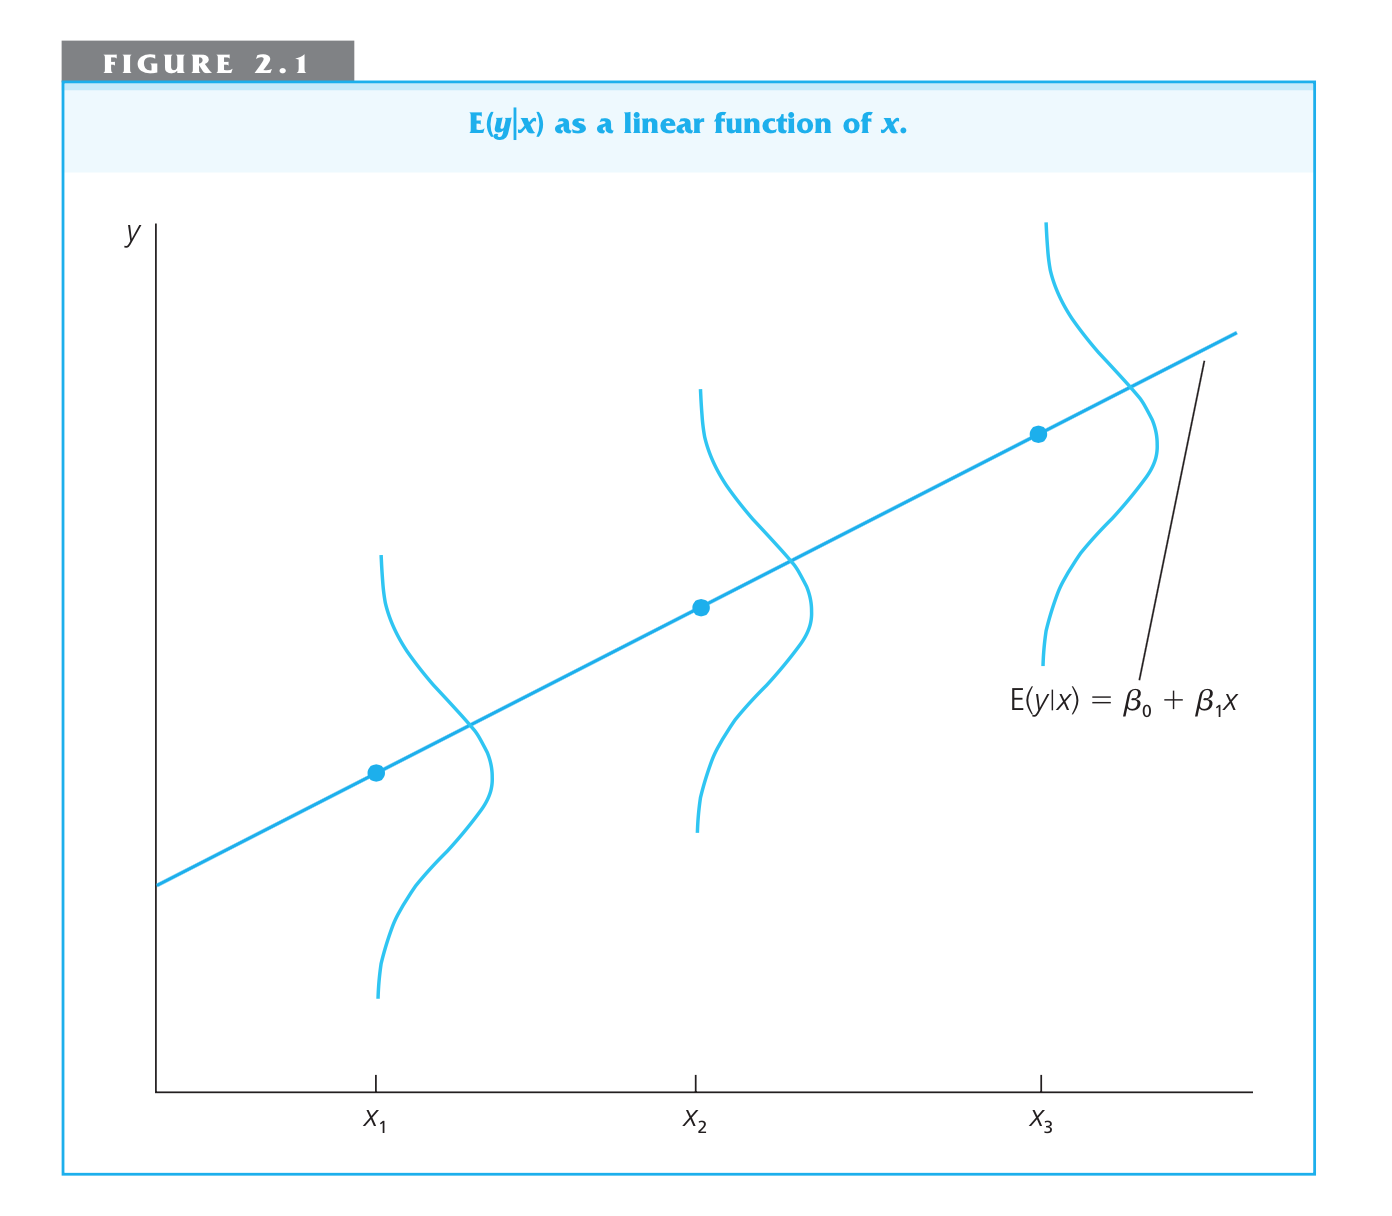
\includegraphics[width=8cm]{5.png}
\end{center}

\end{itemize}
The above assumptions are used to motivate OLS estimators of given a random sample of data. 

\subsection{Derive OLS estimator from assumptions}

There are several ways to motivate the following estimation procedure. We will use zero mean assumption and an important implication of zero conditional mean assumption: \\

\begin{center}

    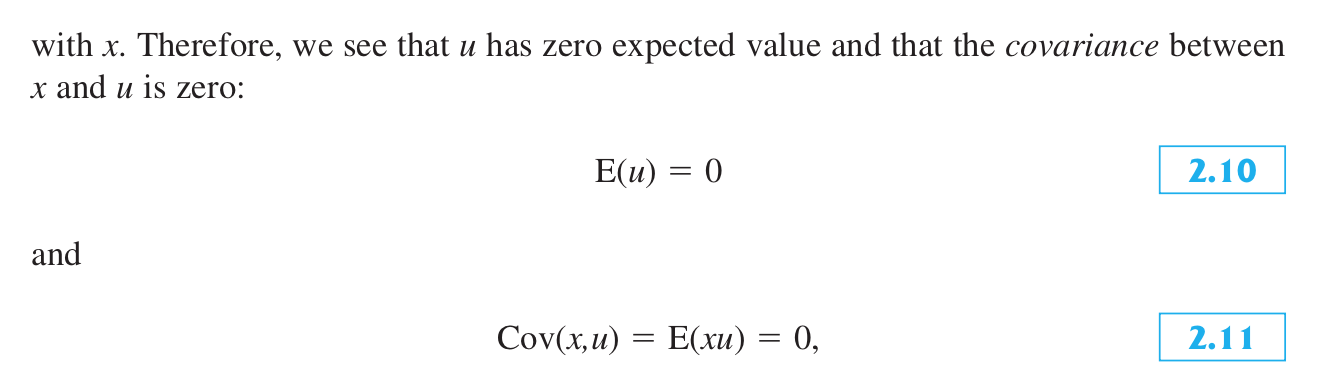
\includegraphics[width=8cm]{6.png}
\end{center}

Then change the above equations in terms of the observable variables x and y and the unknown weight vector $\theta$:\\

\begin{center}

    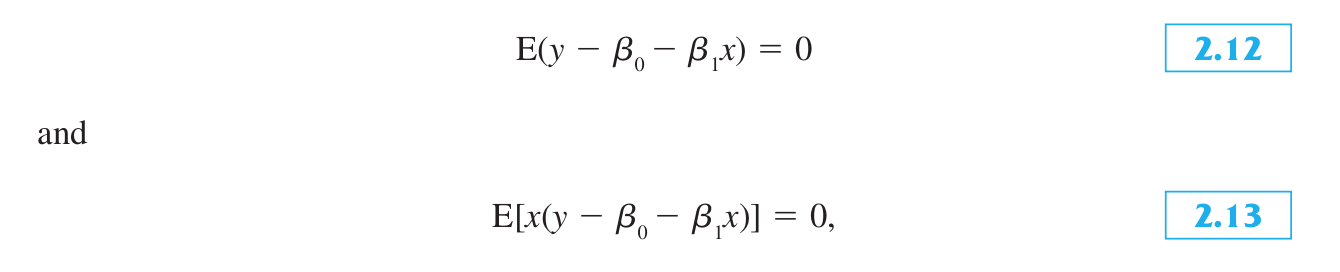
\includegraphics[width=8cm]{7.png}
\end{center}


\begin{center}

    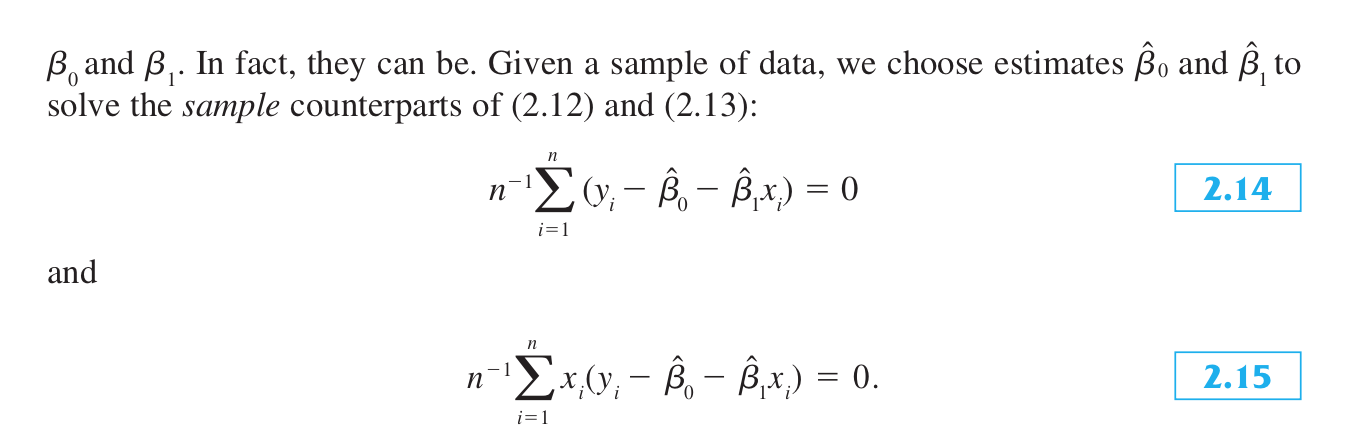
\includegraphics[width=8cm]{8.png}
\end{center}

In multivariate case, the equation is expressed as below:\\

\begin{equation}
    \frac{1}{N} \sum_{i=1}^{N} (y_{i}-\bar{\theta}\tran x_{i})=0
\end{equation}    
   
   
   
\begin{equation}
    \frac{1}{N} \sum_{i=1}^{N} x_{ik}(y_{i}-\bar{\theta}\tran x_{i})=0 , \forall k
\end{equation} 


which is exactly the first order conditions of the unconstrained optimization problem:$\underset{\theta}{min} \sum_{i=1}^{N} (y^{i}-\theta^{T}x^{i})^2$. So that means, if we can select input variables that can fit the zero mean assumptions and zero conditional mean assumptions, then it naturally meet the OLS requirements, so we can get unbiased estimator.\\

\subsection{statistical properties of OLS estimator}
Homoskedasticity:\\
that is:\\
$var(\epsilon|x)=\sigma^2$ for univariate case\\
And $var(\epsilon|x)=\Sigma$ for multivariate case\\
We must emphasize that the homoskedasticity assumption is quite distinct from the zero conditional mean assumption\\
Why we need the Homoskedasticity assumption?:\\
it is important to know how far we can expect $\bar{\theta}$ to be away from $theta$ on average. Among other things, this allows us to choose the best estimator among all, or at least a broad class of, unbiased estimators. \\
case where the Homoskedasticity is not met:\\

\begin{center}

    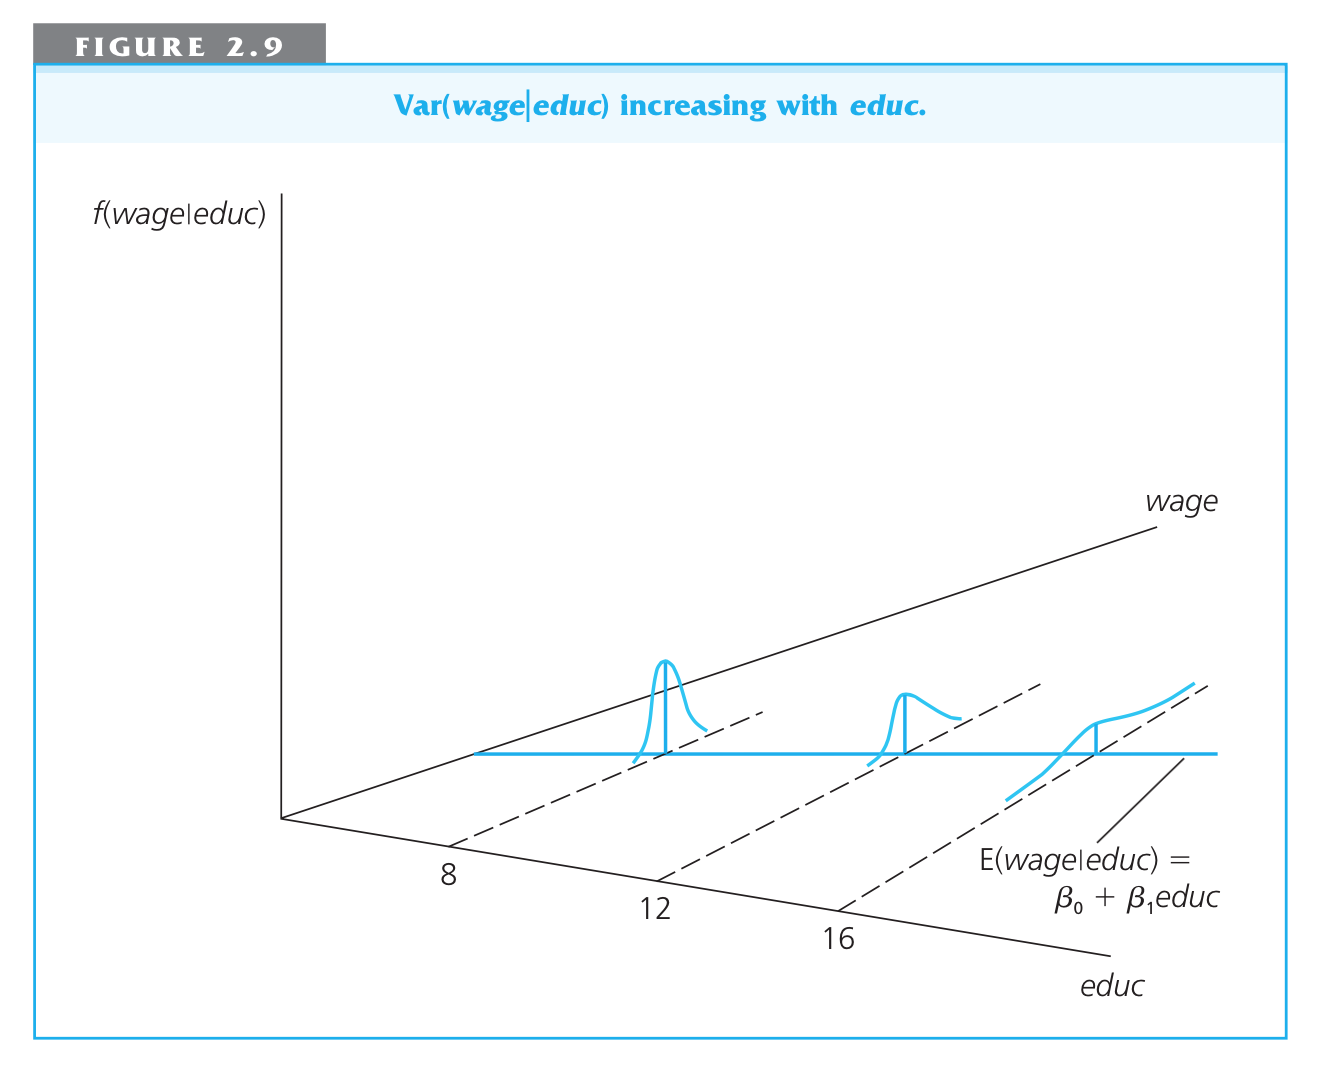
\includegraphics[width=8cm]{9.png}
\end{center}
 


\section{MLE estimator in ML}
\subsection{Notations \& Normal Distribution}
n:dimensions of $x^{i}$\\
N:size of data\\
\\
$ x =\left[ \begin{array}{c} x_{0} \\ x_{1} \\ .\\.\\ x_{n} \end{array} \right] \in R^{n+1}$
$ \Theta =\left[ \begin{array}{c} \Theta_{0} \\ \Theta_{1} \\ .\\.\\ \Theta_{n} \end{array} \right] \in R^{n+1}$\\
$y = \theta^{T}x +\epsilon$ where $\epsilon \sim \mathcal{N}(0,\Sigma)$\\
Then:\\
$y^{i} = \theta^{T}x^{i} +\epsilon$ where $\epsilon \sim \mathcal{N}(0,\Sigma)$\\
Then:\\
$P(y^{i}|\theta,x^{i},\Sigma)=N(\theta^{T}x^{i},\Sigma)$\\
Then:\\
$P(y|\theta,X,\Sigma) = \prod_{i=1}^{N} P(y^{i}|\theta,x^{i},\Sigma)$\\


If $y^{i} \sim N(\mu^{i},\Sigma)$,then:\\
$P(y^{i}|\mu^{i},\Sigma)=|2\pi\Sigma|^{\frac{1}{2}}exp(-\frac{1}{2}(y^{i}-\mu^{i})^{T}\Sigma^{-1}(y^{i}-\mu^{i}) )$\\

\subsection{\red{Why we do not consider the assumptions problem in ML?}}
In ML we make the strongest assumption that,$\epsilon \sim \mathcal{N}(0,\Sigma)$, and we make the strongest assumption that x and u are independent\\

Then given the above two strongest assumptions, the three assumptions zero mean, zero conditional mean,Homoskedasticity will naturally met.\\

\subsection{MLE = OLS in ML framework assumptions}
Typically we can use MLE and least sqaure method to compute $\mu$, both of which in the end are optimization problems\\
We here need to prove that the two method are in essence the same:\\
$Ln(P(y|\theta,X,\sigma^2))=\sum_{i=1}{N} Ln(P(y^{i}|\theta,x^{i},\sigma^2))= \sum_{i=1}^{N} Ln(N(y^{i}|\theta,x^{i},\sigma^2))$\\
$=\sum_{i=1}^{N} [-\frac{1}{2}Ln(2\pi\sigma^2)]-[\frac{1}{2\sigma^2}\sum_{i=1}^{N} (y^{i}-\theta^{T}x^{i})^2]$\\

Then $\underset{\theta}{min}L(\theta)$ is identical to $\underset{\theta}{min} \frac{1}{2}\sum_{i=1}^{N} (y^{i}-\theta^{T}x^{i})^2$\\


\subsection{Difference}

Economics deal with variable selection, and interpreting the weights,and naturally how to deal with the situations where the three assumptions do not hold(also random sampling is another assumption that should be met, when it is not satisfied, certain methods shall be used).There we need intuition of economic phenomena as well as some interpretation of data analysis result of different regression models\\

And machine learning \cite{friedman2001elements} is after the variable selection step, when we have successfully select variables of interest. We improve the models by :(1) just regression-related model:we seek to find the best estimator for prediction, so to prevent over-fitting, we use regularization method;(2) when predicting two variables(input,output) that are macro-variables of an integrated system, it is better to use state-space model, then the framework of MLE framework(or MAP in Bayesian)to convert the parameter estimation(identification) problem into an optimization problem is still applicable. And that is why ML is so powerful.\\







\section{Common problems and methods in Economics when the four assumptions are not satisfies(zero mean, zero conditional mean,
Homoskedasticity, random sampling)}

\subsection{Homoskedasticity is not satisfied  \cite{dandan2013}}

heteroscedasticity problem

\subsection{Random sampling assumption is not satisfied  \cite{dandan2013}}

\subsection{Zero condition mean assumption is satisfied:endogenous problem \cite{dandan2013}}
Types of reason of violation of zero condition mean assumptions:\\
\begin{itemize}
    \item {Functional Form Misspecification}
    \item{Models with Random Slopes}
    \item{Missing variables}
    \item{reverse causality}
\end{itemize}

Possible solutions:\\
\begin{itemize}
    \item {Proxy Variables for Missing variables}
    \item{instrumental variable for all the other cases}
\end{itemize}

\subsection{Week Exdogenity \cite{jackman2009bayesian}}
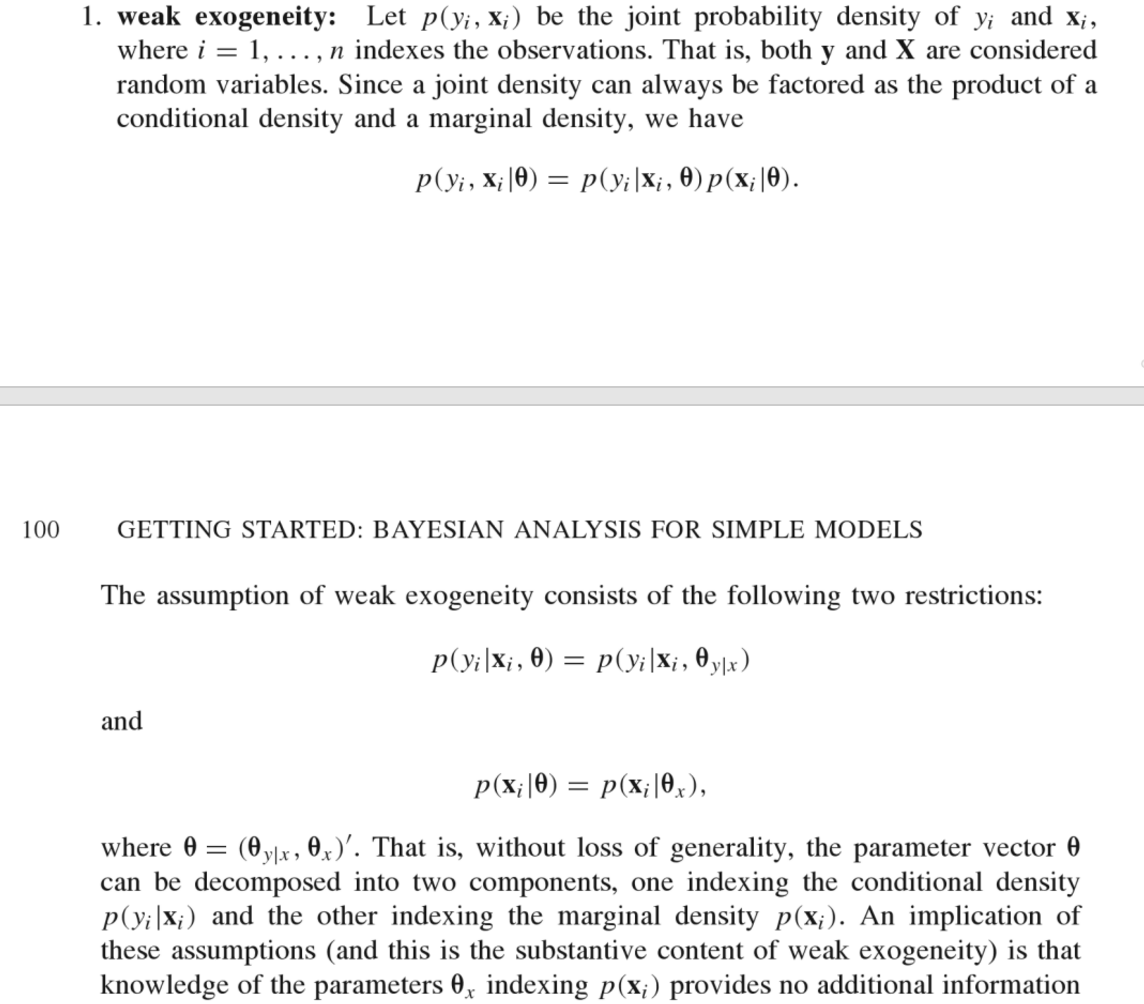
\includegraphics[width=12cm]{3.png}\\





\section{\red{Regression with Time Series Data \cite{wooldridge2015introductory}}}

Part 2: chapter 10-12\\


\begin{center}
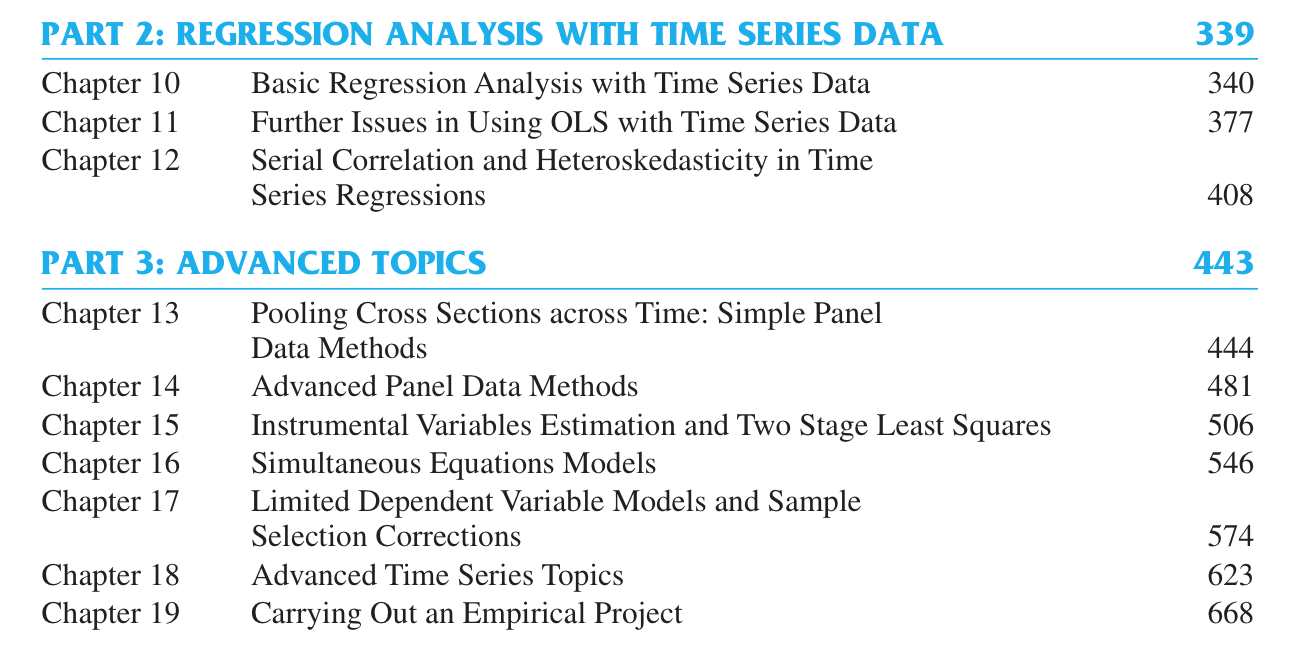
\includegraphics[width=8cm]{10.png}
\end{center}



\section{Formulation of logistics regression}

\subsection{Theorem of EV}

\href{https://en.wikipedia.org/wiki/Generalized_extreme_value_distribution}{\texttt{Generalized Extreme Value Distribution}}

if $\epsilon ~\sim EV(\eta,\mu)$, then $a\epsilon+b ~\sim EV(a\eta+b,\frac{\mu}{a})$, from here we can get the theorem for two competing EV variable, just like two exponentially- distributed variables.\\

\begin{equation}
    If x_{1} \sim exp(\lambda_{1}),x_{2} \sim exp(\lambda_{2}), then: P(x_{1}<x_{2})=\frac{\lambda_{1}}{\lambda{1}+\lambda_{2}}
\end{equation}

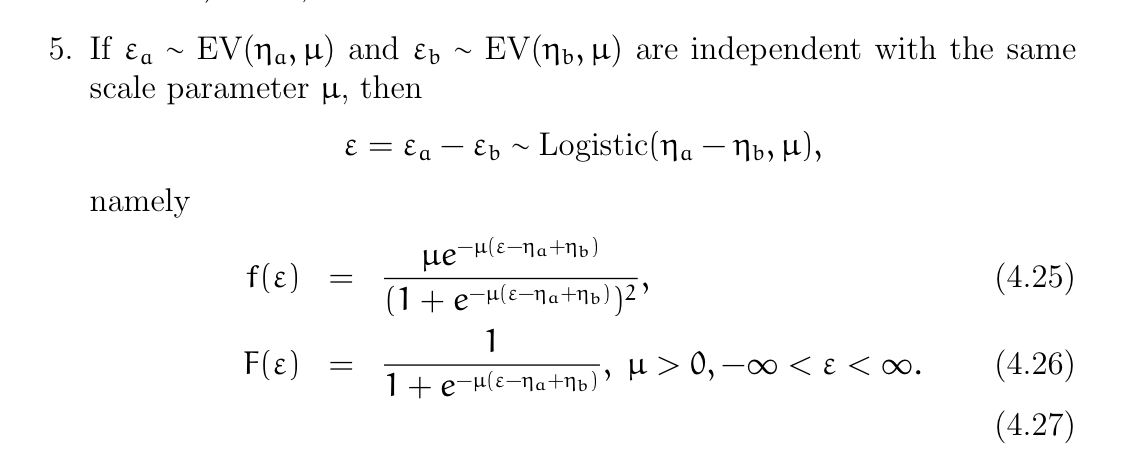
\includegraphics[width=12cm]{1.png}\\
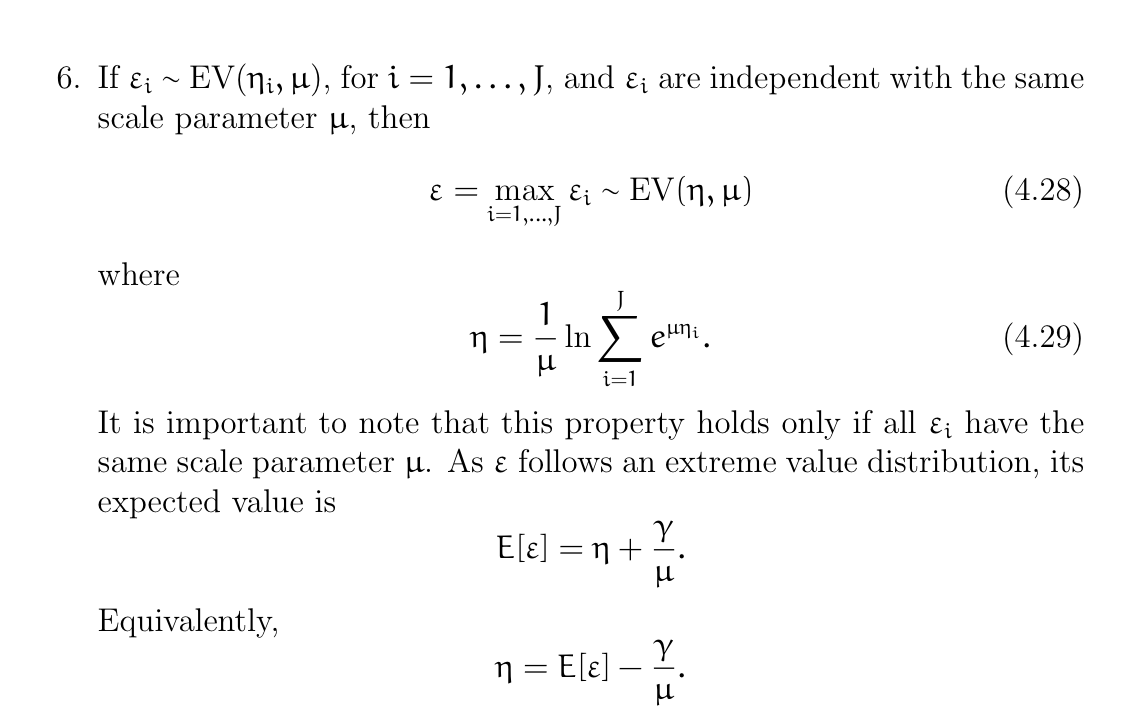
\includegraphics[width=12cm]{2.png}\\


\subsection{from assumption of $\epsilon ~\sim EV(\eta,\mu)$ to expression of $P(t_{i}=1|\theta,b)$, and then to MLE estimation of parameters}


\begin{equation}
    U_{1} = \theta\tran x + b + \epsilon, \epsilon \sim EV(\eta,\mu)\\
\end{equation}

\begin{equation*}
    U_{0}= \epsilon , \epsilon \sim EV(\eta,\mu)
\end{equation*}

Then how to get 
\begin{equation}
 P(t=1) = \frac{\exp(\theta\tran x + b)}{1+\exp(\theta\tran x + b)} 
\end{equation}

from above definition of probabilistic utility function and theorem of EV(extreme values)?\\



\medskip

\bibliography{sample}

\end{document}
